\section{Response Time Functions}\label{RTFs}
%III.	Application Functions
%	a.	Resource Value Functions
%		i.	Structure
%		ii.	Model Building Approach
%			1.	Who measures the data?
%	b.	Penalty Functions
%		i.	Where do the deadlines come from?
%		ii.	How do we set the slopes?
%	c.	Power Model


In this section, we describe the design of \pacora's RTFs in more detail.
RTFs describe an application's performance given its resource assignments.  These functions capture information about the performance impact of a particular resource to an application on the current hardware at a particular time. Without this information, it would be difficult for any resource allocation system to make informed decisions short of blindly trying a variety of allocations and picking the best one.

\subsubsection*{Modeling versus Interpolating} While it might have been possible to model response times by recording past values and interpolating among them, this idea has serious shortcomings:
\begin{itemize}
\item The multidimensional response time tables would be large;
\item Interpolation in many dimensions is computationally expensive;
\item The measurements will be noisy and require smoothing;
\item Convexity in the resources may be violated;
\item Gradient estimation will be slow and difficult.
\end{itemize}

Instead of interpolating, \pacora maintains a parameterized analytic response time model with the partial derivatives evaluated from the model \emph{a priori}. Application responsiveness is highly nonlinear for an increasing variety of applications like streaming media or gaming, thus requiring many data points to represent the response times without a model. Using models, each application can be described in a small number of parameters.  Models can be built from just a few data points and can naturally smooth out noisy data. Their gradients, needed by \pacora to solve the optimization problem efficiently, are easy to calculate.

\pacora models response times with functions that are convex by construction.
The specific function chosen for \pacora is shown in Equation~\ref{rtf_eq} above.
In this equation, the response time is modeled as a weighted sum of component terms,
roughly one per resource, where a term $w_i/a_i$ is the amount of work $w_i \geq 0$
divided by $a_i$, the allocation of the $i$th resource~\cite{Snav}.
For example, one term might model instructions executed divided by total processor MIPS;
another might model network accesses divided by bandwidth, and so forth.
%Asynchrony and latency tolerance may make response time components overlap partly or fully; and thus we added additional terms to represent the interactions between resources.

Such models are automatically convex in the allocations because $1/a$ is convex for positive $a$ and because a positively-weighted sum of convex functions is convex.  The models are also linear in the weights.

%It is obviously important to guarantee the positivity of the resource allocations. This guarantee can be enforced as the %allocations are selected during penalty optimization, or the response time model can be made to return $\infty$ if any allocation %is less than or equal to zero. This latter idea preserves the convexity of the model and extends its domain to all of $\Re^n$ and %consequently we used this approach in our implementation.
%The gradient $\nabla\tau$ is needed by the penalty optimization algorithm.
%Since $\tau$ is analytic, generic, and symbolically differentiable
%it is a simple matter to compute the gradient of $\tau$ once the model is defined.

\subsubsection*{Non-Convexity}
Forcing RTFs to be convex assumes that the actual response times are
close to convex. We find this to be a plausible requirement as
applications usually follow the ``Law of Diminishing Returns'' for
resource allocations.

However, there are examples of response time versus resource behavior that violate convexity.   For example, we have seen non-convex performance in applications when dealing with hyperthreads or memory pages.  For two of our applications, 5 hyperthreads resulted in significantly worse performance than either 4 or 6.  When studying some other applications, we found that particular numbers of memory pages, (\emph{e.g.,} 2K), resulted in much better performance than the adjacent page allocations.  Outliers and additional challenges to response time modeling are discussed in Section~\ref{discuss}.
%Avoiding (or seeking out) these allocations would add significant cost to the optimization problem.

Another kind of convexity violation can occur in memory allocation, where ``plateaus'' can sometimes occur as in Figure~\ref{f:plat}. Such plateaus are typically caused by adaptations within the application (\emph{e.g.,} adjusting the algorithm or output quality).
%to accommodate variable resource availability.  
The response time is really the \emph{minimum} of several convex functions depending on allocation, and the point-wise minimum that the application implements fails to preserve convexity.  The effect of the plateaus will be a non-convex penalty as shown in Figure~\ref{f:plateffect} and multiple extrema in the optimization problem will be a likely result. 



\begin{figure}[hb]
\parbox{1.6in}{
\includegraphics*{Plateau1.eps}
\caption{\label{f:plat}Response time function with some resource ``plateaus''.}
}
\hspace{\fill}
\parbox{1.6in}{
\includegraphics*{Plateau2.eps}
\caption{\label{f:plateffect}Net effect of the resource plateaus on the application penalty.}
}
\end{figure}
There are several ways to avoid this problem.  One is based on the observation that such response time functions will at least be \emph{quasiconvex}.  Another idea is to use additional constraints to explore convex sub-domains of $\tau$. Either approach adds significant computational cost, and we found that our simple convex models still resulted in high-quality resource allocations. Thus we chose not to implement any of these approaches.  Alternative approaches to handling non-convex behavior are described in~\cite{pacora_tr}. 

%\subsubsection*{Dynamically Changing Applications}
%
%
%\fix{changing apps}
%\fix{dynamic compilation}
%\fix{phases}
%Response time will commonly vary with time as a application changes phase and makes better or worse use of its resources.
%\fix{non-determinism}
%
%\fix{Input Variability}


\subsubsection*{Data Collection and Model Creation Time}
There are many ways to collect the response time data for
applications. The user-level runtime scheduler is one possible source,
or the operating system could measure progress using performance
counters.  In our implementation, applications report their own
measured values; however, this solution was chosen simply as a way to
test the validity of the concept.  In a production operating system it
may not be a good idea because applications could lie about their
performance.  In a single-operator datacenter environment this might be less of a concern.

There are also many different possible moments to create response time functions.  RTFs could be created in advance and distributed with the application. This approach could make lots of sense for app stores since most of them cater to just a few platforms. RTFs could also be crowd-sourced and built in the cloud, which has the advantage making it easy to collect a diverse set of training points.  However, all of these approaches lack adaptability.  As a result, we have chosen to implement two solutions that collect data directly from the user's machine.  The first approach is to adapt to the system by collecting all of the training points at application install time and building the model then.  The most highly adaptive approach collects data continuously as the application runs, uses the data to modify the model training set, and rebuilds the model.  A hybrid approach may be the most effective: applications can begin with a generic model and improve it over time. The remainder of this Section describes our model creation process in detail.
\subsection{Response Time Model Creation}
To create RTF models either at install time or online we use a convex
least-squares approach described below.  At install time, we use a
genetic algorithm, Audze-Eglasis Design of
Experiments\cite{bates-aes03}, to select the resource vectors to use
for training.  These vectors and their response times are fed into the
convex least-squares algorithm. Online model building uses data
from the application's response time history.

\subsubsection*{Least-Squares Minimization}
After enough measurements, discovery of the model parameters $w$ that define the function $\tau$
can be based on a solution to the over-determined linear system $t=Dw$,
where $t$ is a column vector of actual response times measured for the application
and $D$ is a matrix whose $i$th row $D_{i,*}$ contains the corresponding resource vector.
Estimating $w$ is relatively straightforward: a least-squares solution accomplished via
\emph{QR factorization}\cite{GoVL} of $D$ will determine the $w$ that minimizes the \emph residual error of
$\|Dw - t\|^2_2 =  \|Rw - Q^Tt\|^2_2$.
%The solution proceeds as follows:
%\begin{eqnarray*}
%t     &=& Dw  - \varepsilon    \\
%      &=& QRw - \varepsilon    \\
%Q^Tt  &=& Rw  - Q^T\varepsilon
%\end{eqnarray*}
%
The individual elementary orthogonal transformations, \emph{e.g.,} Givens rotations,
that triangularize $R$ by progressively zeroing out $D$'s sub-diagonal elements are simultaneously applied to $t$.
%The elements of the resulting vector $Q^Tt$ that correspond to zero rows in $R$ comprise $-Q^T\varepsilon$.
%Since $Rw$ exactly equals the upper part of $Q^Tt$, the upper part of $Q^T\varepsilon$ is zero. The residual error for the %$t_i$
%can be found by premultiplying $Q^T\varepsilon$ by $Q$.

%This formulation assumes a model norm $p = 1$. If a different model norm $p$ is desired, such as $p = 2$, we could first square %each measurement in $t$
%and each reciprocal bandwidth term in $D$ and then follow the foregoing procedure.
%The elements of the result $w$ will be squares as well, and the 2-norm of the difference in the squared quantities will be %minimized.  This is not the same as minimizing the 4-norm; what is being minimized is $1/2\|\mbox{diag}(Dww^TD^T - tt^T)\|^2_2$.

\subsection{On-line Response Time Modeling}
As resource allocation continues, more measurements will become available to augment $t$ and $D$.
Moreover, older data may poorly represent the current behavior of the application.
\pacora uses an incremental approach described below to replace old data and efficiently update RTFs.

\subsubsection*{Incremental Least-Squares}
What is needed is a factorization $\tilde{Q}\tilde{R}$ of a new matrix $\tilde{D}$
derived from $D$ by dropping a row, perhaps from the bottom,
and adding a row, perhaps at the top.
Corresponding elements of $t$ are dropped and added to form $\tilde{t}$.

The matrices $\tilde{Q}$ and $\tilde{R}$ can be generated by applying Givens rotations
as described in Section 12 of \cite{GoVL} to \emph{downdate} or \emph{update} the factorization
much more cheaply than recomputing it \emph{ab initio}.
The method requires retention and maintenance of $Q^T$ but not of $D$.
Every update in \pacora is preceded by a downdate that makes room for it.
Downdated rows are \emph{not} always the oldest (bottom) ones, but
an update always adds a new top row.
For several reasons, the number of rows $m$ in $R$
will be at least twice the number of columns $n$.
Rows selected for downdating will always be in the lower $m - n$ rows of $R$,
guaranteeing that the most recent $n$ updates are always part of the model.

%\subsubsection*{Non-Negativity}
%\begin{figure*}[!t]
%	\begin{center}	
%%		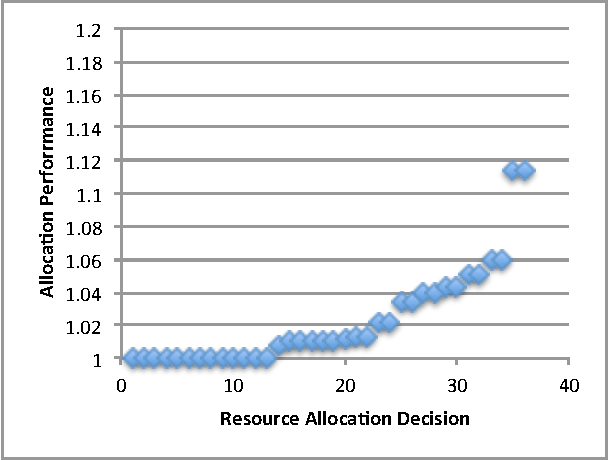
\includegraphics[width=.45\textwidth]{cluster_decision_points.pdf}
%		\caption{Performance of \pacora's NNLS algorithm}
%		\label{model_build_perf}
%	\end{center}
%\end{figure*}

To guarantee convexity of the RTF, the solution $w$ to $t \approx QRw$ must have no negative components.
Intuitively, when a resource is associated with more than a single $w_j$
or when the measured response time increases with allocation then negative $w_j$ may occur. \emph{Non-negative Least-Squares} problems (NNLS) are common linear algebra, and there are several well-known techniques\cite{ChPl}.
However since \pacora's online model maintenance calls for
incremental downdates and updates to rows of $Q^T$, $Q^Tt$ and $R$,
the NNLS problem is handled with a scheme
based on the \emph{active-set} method\cite{LaHa} that
also downdates and updates the \emph{columns} of $R$ incrementally,
roughly in the spirit of Algorithm~3 in~\cite{LuDu}.
However, \pacora's algorithm cannot ignore downdated columns of $R$
because subsequent \emph{row} updates and downdates must have due effect
on these columns to allow their later reintroduction via column updates as necessary.
This problem is solved by leaving the downdated columns in place,
skipping over them in maintaining and using the QR factorization.

The memory used in maintaining a model with $n$ weights is modest, $24n^2 + 21n + \textrm{O}(1)$ bytes.
For $n = 8$ this is under 2 KB, fitting nicely in L1 cache.
Our NNLS implementation takes 4 $\micro$s per update-downdate pair in \tess.
%Figure~\ref{model_build_perf} shows the performance of \pacora's NNLS algorithm.

\subsubsection*{Model Rank Preservation}
If care is not taken in downdating $R$, its rows may become so linearly dependent,
perhaps from repetitive resource allocations,
that determining a unique $w$ is impossible.
The rank of $R$ depends on both the resource optimization trajectory and the
choices made in the row downdate-update algorithm.
\pacora exploits the latter idea and simply avoids downdating any row that will make $R$ rank-deficient.

\subsubsection*{Outliers and Phase Changes}

%\begin{figure*}[!t]
%	\begin{center}	
%%		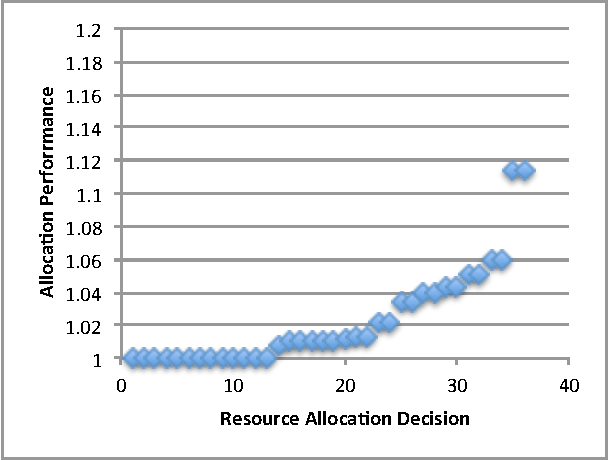
\includegraphics[width=.45\textwidth]{cluster_decision_points.pdf}
%		\caption{\pacora's online model creation algorithm adapting to a video application changing phases}
%		\label{phase_change}
%	\end{center}
%\end{figure*}

Some response time measurements may be ``noisy'' or even erroneous.
A weakness of least-squares modeling is the high importance it gives to outlying values.
On the other hand, when an application changes phase it is important to adapt quickly,
and what looks like an outlier when it first appears may be a harbinger of change.
What is needed is a way to discard either old or outlying data
with a judicious balance between age and anomaly.

The downdating algorithm accomplishes this by weighting the errors in $\varepsilon = Q(Q^Tt - Rw)$
between the predicted response times $\tau$ and the measured ones $t$ by a factor
that increases exponentially with the age $g(i)$ of the error $\varepsilon_i$.
Age can be modeled coarsely by the number of time quanta of some size since the measurement;
\pacora simply lets $g(i) = i$.
The weighting factor for the $i$th row is then $\eta^{g(i)}$ where $\eta$ is a constant somewhat greater than 1.
The candidate row to downdate is the row with the largest weighted error, \emph{i.e.,}
$dd = \arg\max_i |\varepsilon_i| \cdot \eta^{g(i)}$ and that does not reduce the rank of $R$.
%Figure~\ref{phase_change} shows \pacora's model creation algorithm adapting to a video application changing phases.


\subsubsection*{Power Response Modeling}
Recall that we manage power and battery energy with an artificial application named application 0 which receives all resources not allocated to other applications. Application 0's "response time" function is similar to the other applications' RTFs.  The function inputs are resource allocations just as with the other applications.  However, the function output is system power rather than response time.   To create the RTF, system power can be measured directly from on-chip energy counters in systems where they are available or from a power meter.  These models can be built in advance, during a training phase or online while the system runs, just as with the application RTFs.  Alternatively, the model could be part of the operating system's platform-specific information.

Although system power may not be perfectly convex in reality, forcing it to be convex is reasonable because idling a resource should not increase power.  As a result, application 0 still fufills its purpose of keeping applications from using additional resources that have poor performance/power ratios.

